\chapter{Container Isolation}

In questa parte vedremo vari concetti che uniti insieme permetteranno di creare
un ambiente isolato che corrisponderà in tutto e per tutto ad un container docker.

\section{Namespaces}

Se i cgroup controllano le risorse che un processo può utilizzare, allora i
\textit{namespace} controlla ciò che i processi possono vedere, dunque restringe
il numero di risorse visibili ad un dato processo.
La sua origine viene datata al sistema operativo Plan 9 che fu il primo ad
introdurle ed usare.
Oggigiorno ci sono molti tipi di namespace supportati da linux:

\begin{itemize}
    \item Unix Timesharing System (UTS)
    \item Process IDs
    \item Mount Points
    \item Network
    \item User and group IDs
    \item Inter-process Communications (IPC)
    \item Control Groups (cgroups)
\end{itemize}

Un processo è sempre esattamente in un namespace di ogni tipo.
Quando linux viene avviato ha un solo namespace per ogni tipo, ma come vedremo
a breve è possibile crearne di nuovi ed aggiungergli processi.\\

È possibile vedere tutti i namespace nella propria macchina con il comando
\verb|lsns|.

\begin{figure}[H]
    \centering
    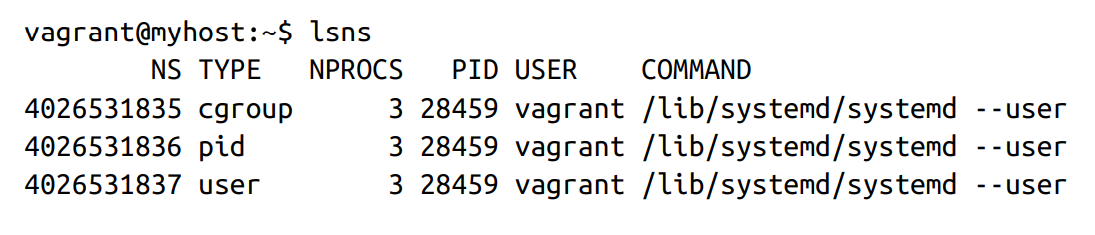
\includegraphics[width=\textwidth, keepaspectratio]{capitoli/os_security/imgs/namespace1.png}
\end{figure}

Eseguire il precedente comando senza i privilegi di root non fornisce tutta la lista
completa dei namespace e dunque per vederli tutti sarà necessario eseguire il comando
con \verb|sudo|.

\begin{figure}[H]
    \centering
    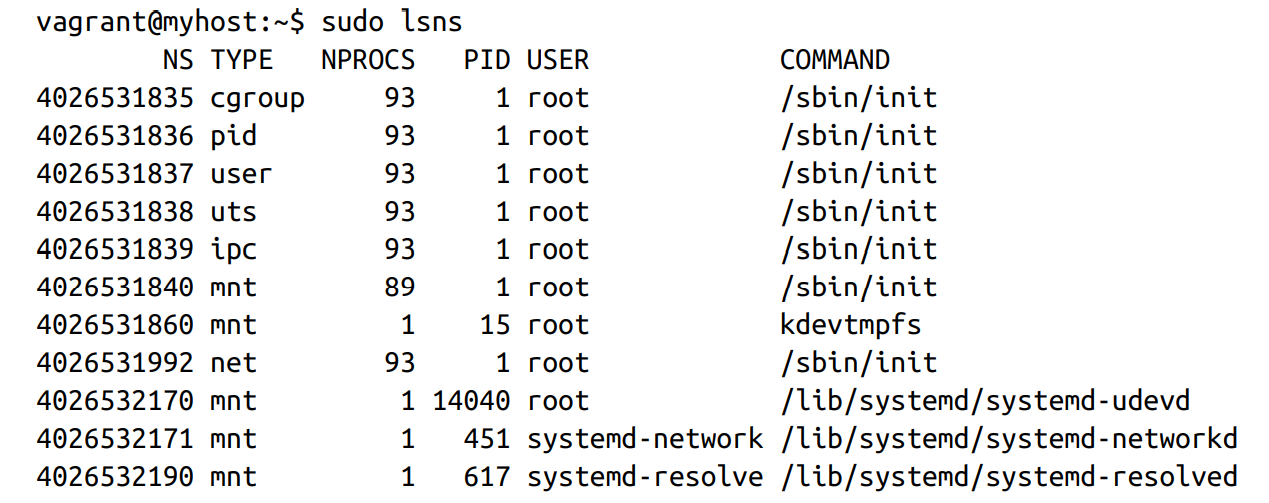
\includegraphics[width=\textwidth, keepaspectratio]{capitoli/os_security/imgs/namespace2.png}
\end{figure}

Vediamo ora come è possibile utilizzare i namespace per creare qualcosa che si
comporti come un container.

\section{Isolare l'Hostname}

Partiamo dal namespace UTS, questo permette di cambiare l'hostname di un processo
indipendentemente da quello della macchina (isola l'hostname).
Un esempio pratico di questo sono i container docker che hanno un proprio hostname
(generalmente l'ID che docker crea automaticamente ad ogni container) diverso da
quello del resto del sistema.

\begin{figure}[H]
    \centering
    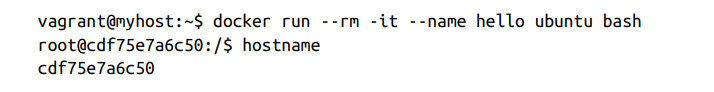
\includegraphics[width=\textwidth, keepaspectratio]{capitoli/os_security/imgs/hostname1.png}
\end{figure}

Docker riesce ad ottenere questo perché crea il suo UTS namespace.
È possibile ottenere un comportamento simile con il comando \verb|unshare| e creare
un processo con il suo UTS namespace.\\

Il comando \verb|unshare| permette di "eseguire un programma con alcuni namespace
separati dal processo padre". Quando un programma viene lanciato, il kernel crea un
nuovo processo e ci esegue il codice del programma. Questa creazione parte dal
contesto di un processo, chiamato \textit{padre}, e
genera un nuovo processo chiamato \textit{figlio}. La parola "unshare" sta ad indicare
il fatto che invece che condividere il namespace del padre, il figlio ne avrà uno tutto suo.
Proviamo ad ottenere questo comportamento, avremmo bisogno dei permessi root,
quindi il comando andrà eseguito come \verb|sudo|.

\begin{figure}[H]
    \centering
    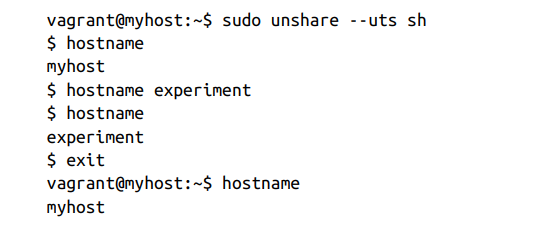
\includegraphics[width=10cm, keepaspectratio]{capitoli/os_security/imgs/hostname2.png}
\end{figure}

Il comando precedente avvia la shell \verb|sh| in un nuovo processo con il proprio
UTS namespace. Possiamo notare che cambiando l'hostname in questo processo
non va a modificare quello del resto del sistema. Se apriamo un altro terminale
prima del comando \verb|exit| possiamo notare come l'hostname non è stato
modificato. Grazie all'UTS namespace possiamo
cambiare l'hostname dell'host senza intaccare quello del processo e viceversa.\\

I namespace sono una componente chiave del funzionamento dei container in quanto
permettono di assegnargli un set di risorse indipendenti dal resto del sistema host
e dagli altri container.

\section{Isolare i Process ID}

Vediamo ora come poter far vedere ad un container solo i processi che ha avviato e
non tutti quelli del sistema host.
In un container docker possiamo vedere solo i processi che girano al suo interno
senza avere accesso a tutti gli altri dell'host. Cerchiamo di raggiungere lo
stesso risultato. Possiamo usare ancora il comando \verb|unshare| specificando
che vogliamo un nuovo PID namespace con il flag \verb|--pid|:


\begin{figure}[H]
    \centering
    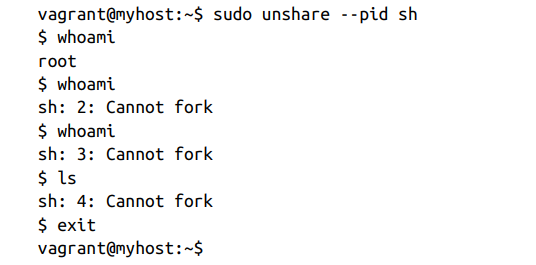
\includegraphics[width=10cm, keepaspectratio]{capitoli/os_security/imgs/pid1.png}
\end{figure}

Non sembra funzionare correttamente ma qualcosa ha fatto, analizziamolo.
Il primo comando sembra aver funzionato correttamente, ma dal secondo in poi
otteniamo un errore. Possiamo notare che gli errori sono formattati nel seguente modo:
\verb|<command>: <process ID>: <message>|. Dal secondo in poi notiamo che i PID
stanno incrementando e possiamo supporre che il PID del primo comando sia 1. Quindi
in un certo modo abbiamo ottenuto quello che volevamo.\\
Per risolvere questo problema ci viene in aiuto il manuale di \verb|unshare| che ci
suggerisce di utilizzare il flag \verb|--fork|: "effettua il fork del programma
specificato come processo figlio di unshare invece di eseguirlo direttamente".
Per come abbiamo eseguito il comando ora abbiamo la seguente situazione:

\begin{figure}[H]
    \centering
    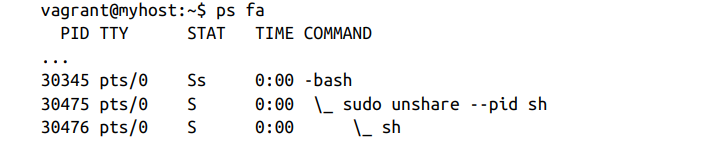
\includegraphics[width=12cm, keepaspectratio]{capitoli/os_security/imgs/pid2.png}
\end{figure}

Notiamo come il processo \verb|sh| non è figlio di \verb|unshare| ma del processo
\verb|sudo|.\\

Proviamo con il nuovo flag:

\begin{figure}[H]
    \centering
    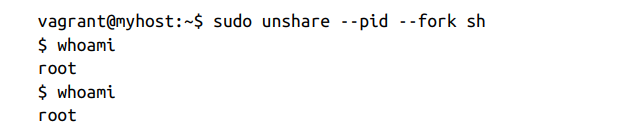
\includegraphics[width=12cm, keepaspectratio]{capitoli/os_security/imgs/pid3.png}
\end{figure}

Ora funziona correttamente. Possiamo eseguire più comandi in successione ed
analizzando la situazione attuale abbiamo:

\begin{figure}[H]
    \centering
    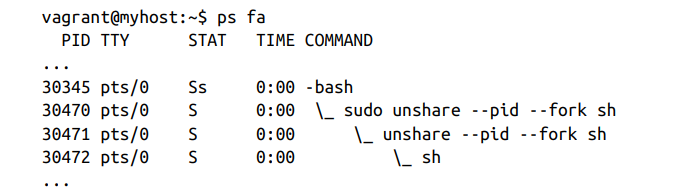
\includegraphics[width=12cm, keepaspectratio]{capitoli/os_security/imgs/pid4.png}
\end{figure}

Eseguendo il comando \verb|ps| all'interno del container ci accorgiamo che
possiamo comunque vedere tutti i processi dell'host anche se ci troviamo
in un nuovo namespace.

\begin{figure}[H]
    \centering
    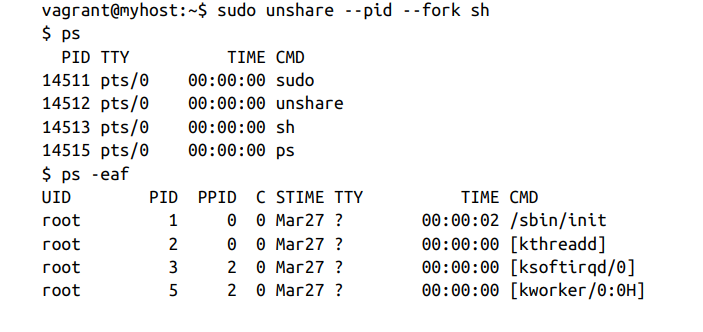
\includegraphics[width=12cm, keepaspectratio]{capitoli/os_security/imgs/pid5.png}
\end{figure}

Questo avviene perché \verb|ps| legge i file virtuali contenuti nella cartella
\verb|/proc|. Andiamo a vedere ora il contenuto di questa directory.

\begin{figure}[H]
    \centering
    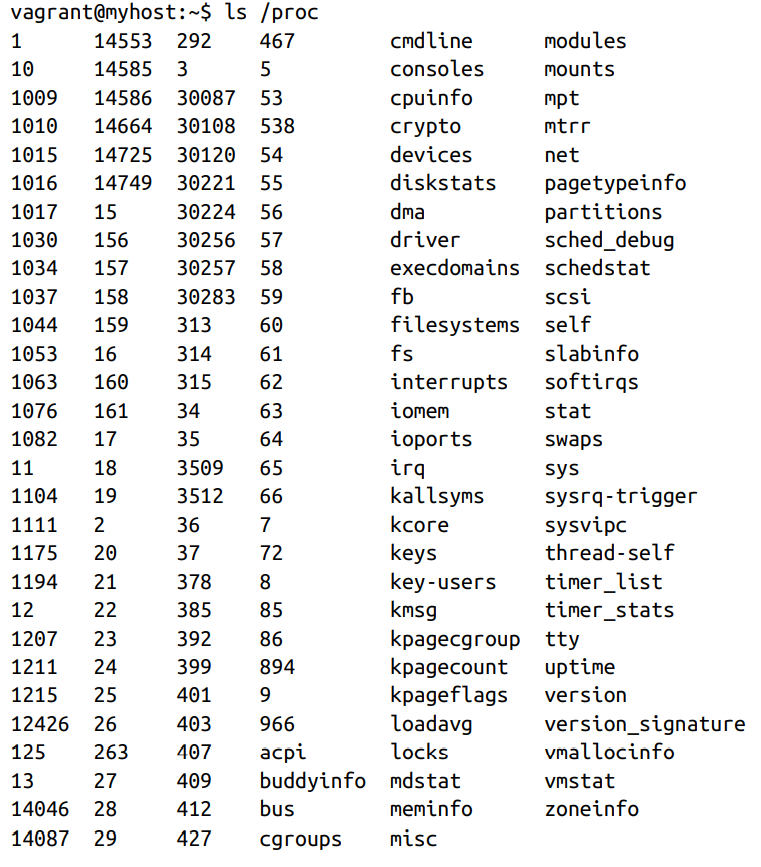
\includegraphics[width=12cm, keepaspectratio]{capitoli/os_security/imgs/pid6.png}
\end{figure}

Ogni directory numerata all'interno di \verb|/proc| corrisponde ad un Process ID,
che contiene molte informazioni riguardante il processo. Per esempio il file
\verb|/proc/<pid>/exe| è un \textit{link simbolico} all'eseguibile del processo
con pid \verb|<pid>|.

\begin{figure}[H]
    \centering
    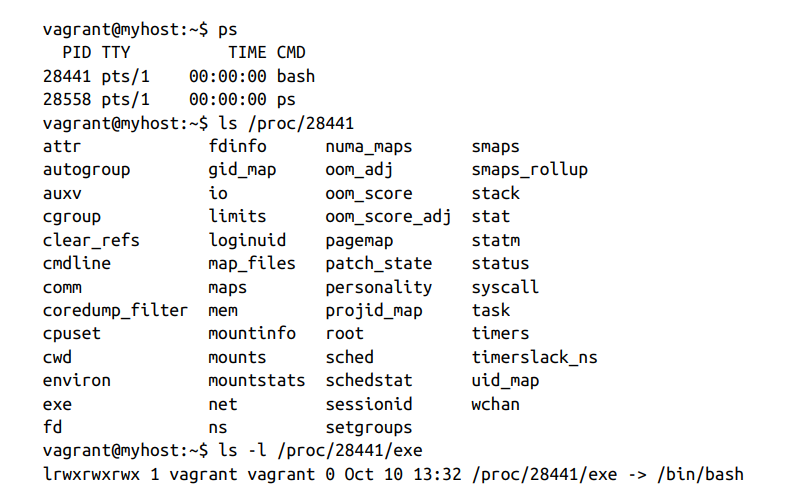
\includegraphics[width=12cm, keepaspectratio]{capitoli/os_security/imgs/pid7.png}
\end{figure}

Dunque per far si che \verb|ps| mostri solo i processi all'interno del nuovo
namespace servirà una copia della directory \verb|/proc| in cui il kernel
potrà scrivere le informazioni riguardanti i nuovi processi e dato che
\verb|/proc| si trova sotto root, questo implica cambiare la directory di root.

\section{Cambiare Root Directory}

La directory di root può essere cambiata con il comando \verb|chroot| e
una volta effettuato questo comando si perde l'accesso ad ogni cosa che si trova
al di sopra della nuova directory di root nella gerarchia del file system.

\begin{figure}[H]
    \centering
    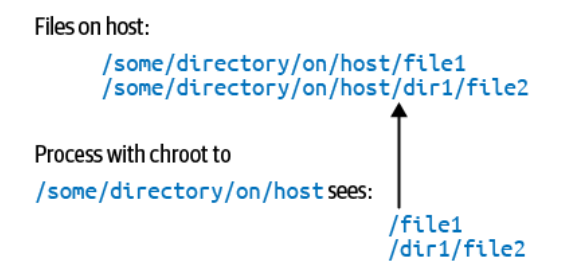
\includegraphics[width=10cm, keepaspectratio]{capitoli/os_security/imgs/root1.png}
\end{figure}

Va fatto notare che quando si va a cambiare la directory di root si perdono anche
tutti gli eseguibili che sia hanno a disposizione solitamente in linux. Sarà
dunque necessario copiare questi file nella nuova directory di root che è
quello che viene effettuato da docker quando istanzia l'immagine del container.

\begin{figure}[H]
    \centering
    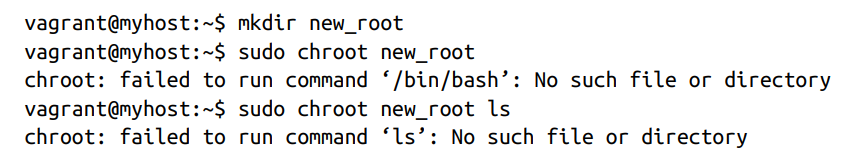
\includegraphics[width=\textwidth, keepaspectratio]{capitoli/os_security/imgs/root2.png}
\end{figure}

\section{Combinare Namespace con Chroot}

% oggi abbiamo visto il mucco (reddit)
È possibile combinare il namespacing e il cambio di root utilizzando \verb|chroot|
in un nuovo namespace. Ora se andiamo a creare una copia della directory
\verb|/proc| situata nel nuovo namespace riusciremo nell'intento precedente
di vedere solo i processi all'interno del nuovo namespace ottenendo così un
isolamento dei processi del container. Questo è possibile perché, come detto
in precedenza, \verb|/proc| è situato nella directory di root quindi creandone una
nuova si può creare una copia indipendente dalla directory originale.
Questo è possibile tramite il seguente comando che dice al container di montare
la cartella \verb|/proc| come uno pseudo-filesystem di tipo \verb|proc|
(gli dice che i processi andranno scritti in quella cartella).

\begin{figure}[H]
    \centering
    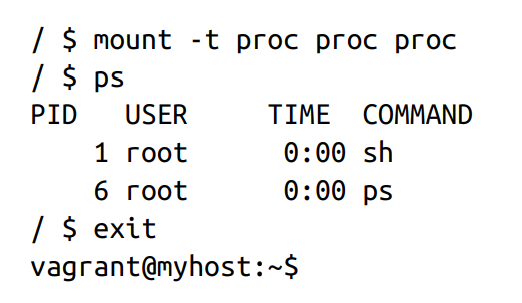
\includegraphics[width=8cm, keepaspectratio]{capitoli/os_security/imgs/insieme1.png}
\end{figure}

\section{Mount Namespace}

Di solito i container hanno un filesystem separato da quello dell'host e per
ottenere questa separazione il container deve avere il proprio
\textit{mount namespace}. Per creare questo nuovo namespace si può utilizzare
il comando \verb|unshare| con il flag \verb|--mount|.

\begin{figure}[H]
    \centering
    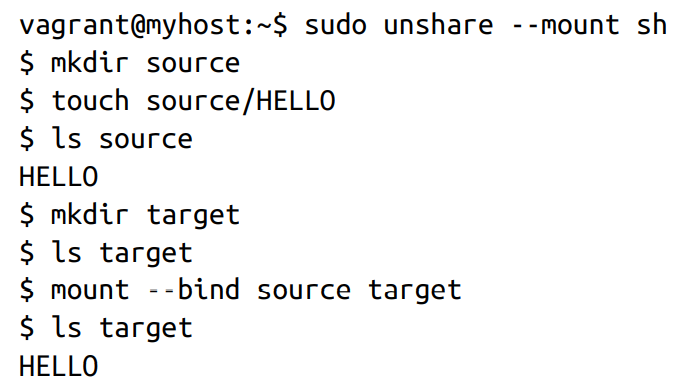
\includegraphics[width=10cm, keepaspectratio]{capitoli/os_security/imgs/mount1.png}
\end{figure}

Dopo aver creato il nuovo mount namespace se si esegue il comando \verb|findmnt|
senza alcun parametro, vedremmo una lunga lista di altri mount, questo perché,
come per i processi, il kernel utilizza ua sottodirectory di \verb|/proc|.
Dunque per ottenere un isolamento totale sarà necessario combinare il nuovo mount
namespace con una nuova root per il filesystem utilizzando \verb|chroot|.

\begin{figure}[H]
    \centering
    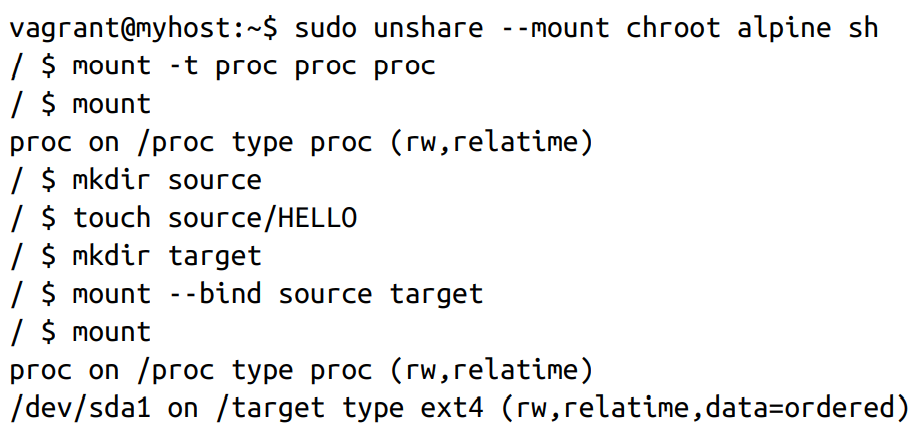
\includegraphics[width=10cm, keepaspectratio]{capitoli/os_security/imgs/mount2.png}
\end{figure}

Nel precedente esempio utilizziamo Alpine Linux come file system e questo non
ha a disposizione il comando \verb|findmnt|, quindi usiamo \verb|mount| senza
parametri che fa la stessa cosa.\\

Se il mount del container è visibile all'host ed il processo del container viene
terminato, sarà necessario eseguire il comando \verb|unmount| perché non viene
automaticamente pulito quando il processo termina, lo stesso vale per \verb|/proc|.
Non è una cosa critica per la sicurezza ma permette di tenere il sistema in ordine.

\section{Network Namespace}

Il \textit{network namespace} permette ad un container di avere la propria visione
delle interfacce di rete e delle \textit{routing table}.
Si può creare un processo con il proprio namespace utilizzando il comando
\verb|unshare| con il flag \verb|--net|.
È possibile vedere tutti i processi che hanno un proprio namespace tramite
il comando\verb|lsns|.

\begin{figure}[H]
    \centering
    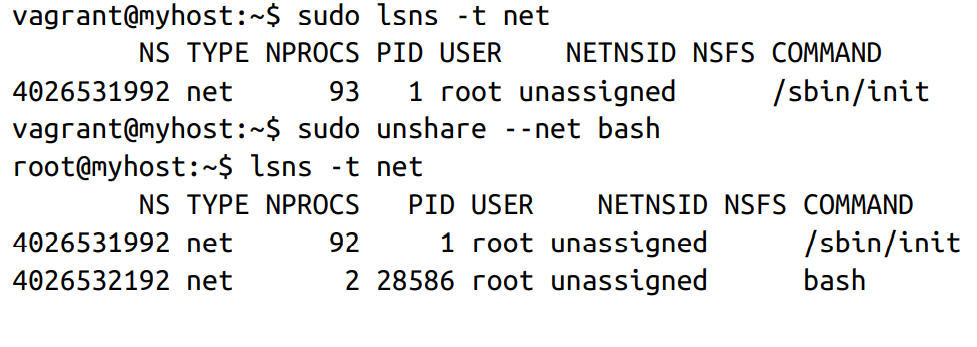
\includegraphics[width=10cm, keepaspectratio]{capitoli/os_security/imgs/net1.png}
\end{figure}

Quando un processo viene messo nel suo network namespace vedrà solamente l'interfaccia
di \textit{loopback} e quindi non sarà in gradi di comunicare con niente.

\begin{figure}[H]
    \centering
    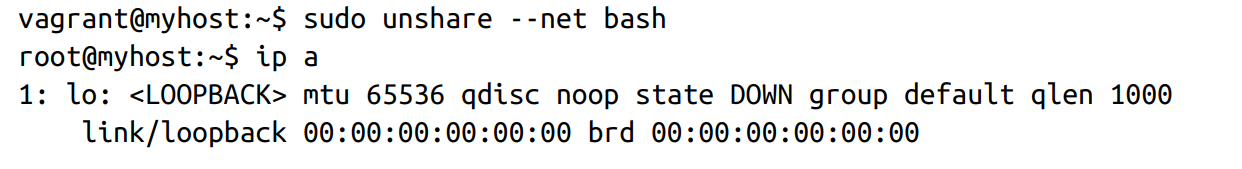
\includegraphics[width=12cm, keepaspectratio]{capitoli/os_security/imgs/net2.png}
\end{figure}

Per permettere al container di comunicare con l'esterno è possibile utilizzare
il seguente comando per creare una sorta di "cavo ethernet virtuale" che connette
il container con l'host.

\begin{figure}[H]
    \centering
    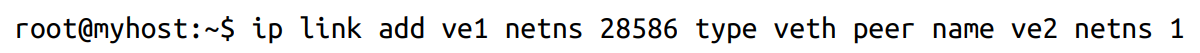
\includegraphics[width=12cm, keepaspectratio]{capitoli/os_security/imgs/net3.png}
\end{figure}

\begin{itemize}
    \item \verb|ip link add|: indica che vuoi aggiungere un link,
    \item \verb|ve1|: il nome di uno dei capi del cavo ethernet virtuale,
    \item \verb|netns 28586|: dice che questo cavo del cavo è inserito nel
          network namespace associato al PID 2856 ,
    \item \verb|type veth|: dice che è una coppia ethernet virtuale,
    \item \verb|peer name ve2|: il nome dell'altro cavo del capo,
    \item \verb|netns 1|: specifica che il secondo capo del cavo è inserito nel
          network namespace associato al PID 1.
\end{itemize}

Ora l'interfaccia \verb|ve1| sarà visibile all'interno del container.

\begin{figure}[H]
    \centering
    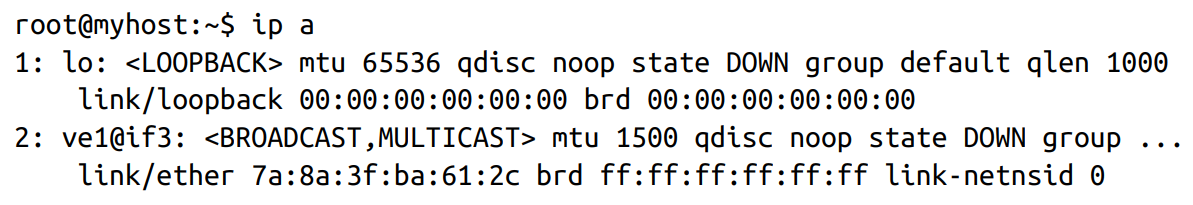
\includegraphics[width=12cm, keepaspectratio]{capitoli/os_security/imgs/net4.png}
\end{figure}

Possiamo notare che la nuova interfaccia è \textbf{DOWN} e deve essere attivata
prima di poterla utilizzare. Questa operazione va effettuata da tutti e due i
"capi" del cavo (sia nel container che nell'host).

\begin{figure}[H]
    \centering
    
\includegraphics[width=8cm, keepaspectratio]{capitoli/os_security/imgs/net5.png}
    \caption{Comando da eseguire nell'host.}
\end{figure}

\begin{figure}[H]
    \centering
    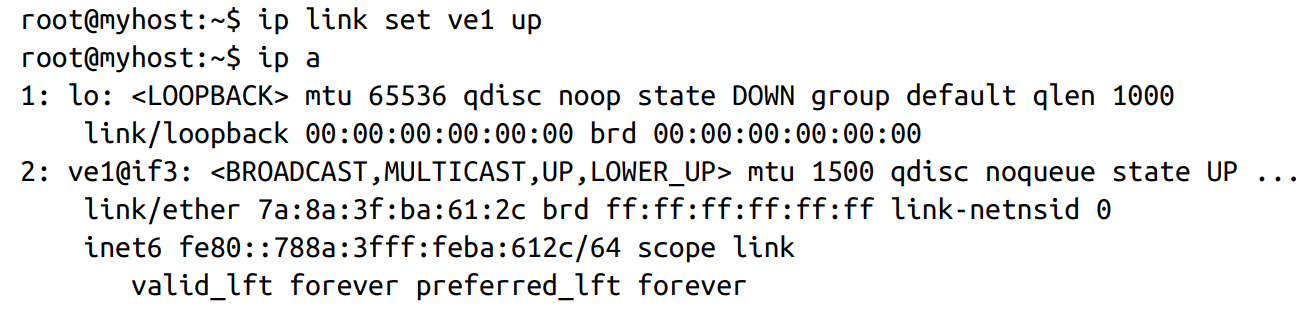
\includegraphics[width=12cm, keepaspectratio]{capitoli/os_security/imgs/net6.png}
    \caption{Comando da eseguire nel container.}
\end{figure}

Come ultima cosa è necessario associare a queste interfacce un indirizzo IP.

\begin{figure}[H]
    \centering
    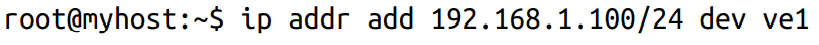
\includegraphics[width=12cm, keepaspectratio]{capitoli/os_security/imgs/net7.png}
    \caption{Comando da eseguire nel container.}
\end{figure}

\begin{figure}[H]
    \centering
    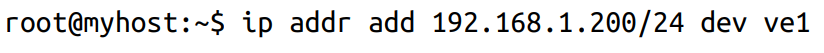
\includegraphics[width=12cm, keepaspectratio]{capitoli/os_security/imgs/net8.png}
    \caption{Comando da eseguire nell'host.}
\end{figure}

\section{User Namespace}

L'user namespace permette ai processi di avere la propria visione degli id dei
gruppi e degli utenti. Il beneficio principale di questo è che si può mappare
l'ID di root (0) all'interno del container, con un'altra identità non-root
all'interno dell'host. Questo è un grande vantaggio nella sicurezza poiché
permette di evitare che un possibile attacco di privilege escalation, faccia ottenere
anche i permessi di root all'interno dell'host.

\begin{figure}[H]
    \centering
    
\includegraphics[width=\textwidth, keepaspectratio]{capitoli/os_security/imgs/user1.png}
\end{figure}

È possibile creare un processo con il proprio user namespace tramite il comando
\verb|unshare| con il flag \verb|--user|.

\begin{figure}[H]
    \centering
    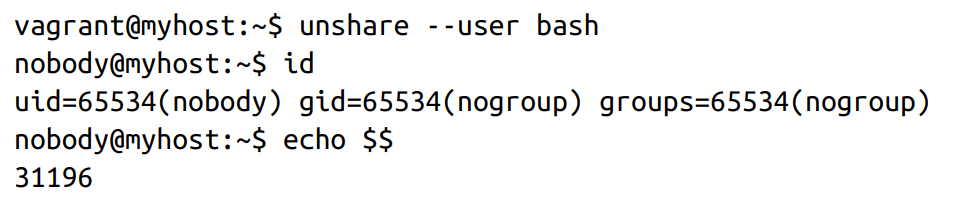
\includegraphics[width=\textwidth, keepaspectratio]{capitoli/os_security/imgs/user2.png}
\end{figure}

Inseguito è necessario effettuare il mapping tra i due ID con il seguente comando:

\begin{figure}[H]
    \centering
    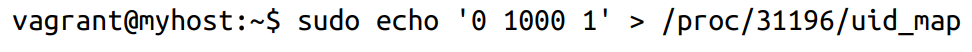
\includegraphics[width=\textwidth, keepaspectratio]{capitoli/os_security/imgs/user3.png}
\end{figure}

Quando viene creato un nuovo processo con il proprio user namespace, il kernel
dà tutte le capabilities al nuovo utente root (pseudo-root user) in modo tale che
sia possibile creare altri namespace. Possiamo vedere questo comportamento in atto
nel seguente esempio:

\begin{figure}[H]
    \centering
    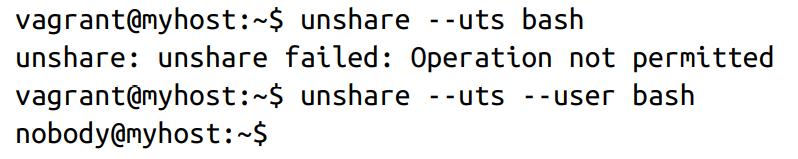
\includegraphics[width=10cm, keepaspectratio]{capitoli/os_security/imgs/user4.png}
\end{figure}

Questo permette di eseguire container con un metodo chiamato \textit{rootless container}
che risulta essere un grande vantaggio dal punto di vista della sicurezza.

\section{Inter-Process Communications (IPC) Namespace}

In linux è possibile comunicare tra processi diversi dandogli accesso ad un'area
di memoria condivisa o utilizzando un coda di messaggi condivisa (queue).
Questi due processi devono essere membri dello stesso IPC namespace per avere
accesso agli stessi identificatori per questi meccanismi.
In generale non si vuole che un container sia in gradi di accedere a della memoria
condivisa che non gli appartiene quindi gli vengono dati i propri IPC namespace.
Per ottenere questo utilizziamo il comando \verb|unshare| con il flag \verb|--ipc|.

\begin{figure}[H]
    \centering
    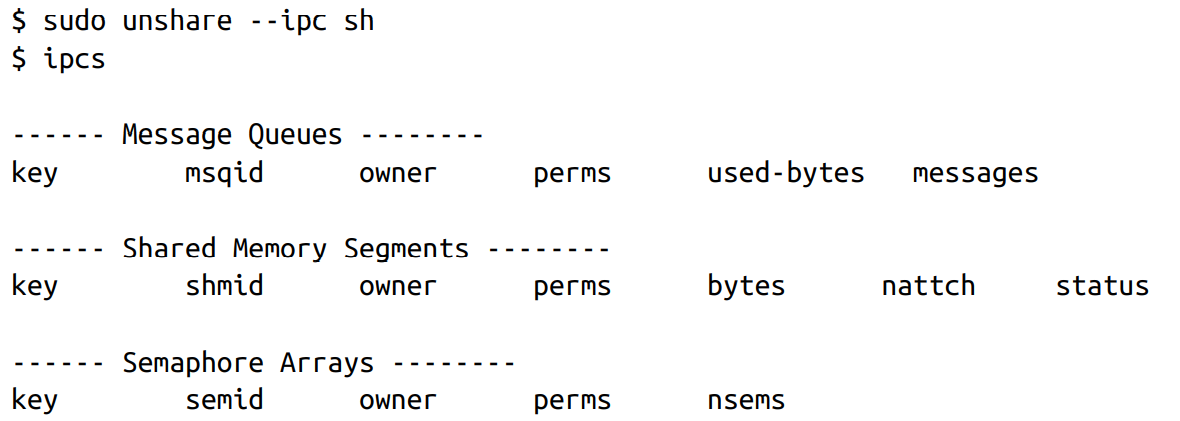
\includegraphics[width=10cm, keepaspectratio]{capitoli/os_security/imgs/user5.png}
    \caption{Esempio di ipc namespace. \textbf{Notare} che senza un IPC separato
        i campi dell'output ipcs risulterebbero essere popolati.}
\end{figure}

\section{Cgroup Namespace}

Questo ultimo namespace impedisce a un processo di vedere le configurazioni di
cgroup che si trovano più in alto nella gerarchia del cgroup directory relativa
a quella del processo in questione. È possibile creare un processo con il proprio
cgroup namespace tramite il comando \verb|unshare| con il flag \verb|--cgroup|.

\begin{figure}[H]
    \centering
    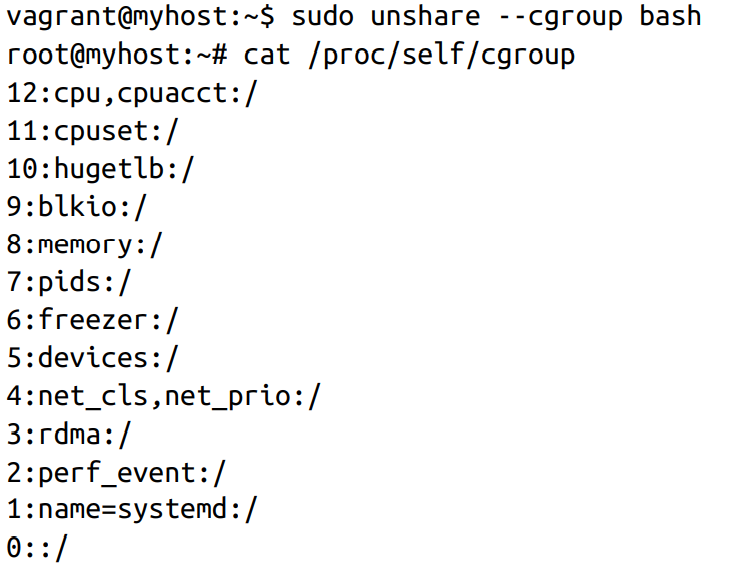
\includegraphics[width=10cm, keepaspectratio]{capitoli/os_security/imgs/cspace.png}
\end{figure}